\section{Algorithm and Empirical Validation}

\subsection{Algorithm \textsc{PlateauRecover}}
\label{sec:algorithm}

Theorem~\ref{thm:headline-formal} is constructive. Each piece of the
estimator $\rhohat$ in~\eqref{eq:headline-estimator} is computable from
the JEPA training trajectory and (on the negative branch) the
sample covariances.
We package the construction as Algorithm~\ref{alg:plateau-recover}.

\begin{figure}[tp]
\centering
\begin{tikzpicture}
\node[anchor=north west, inner sep=0pt] (alg) at (0,0) {%
\begin{minipage}{0.48\linewidth}
\footnotesize
\noindent\rule{\linewidth}{0.4pt}\par\vspace{0.3em}
\textbf{Algorithm 1\;:\;\textsc{PlateauRecover}.}
\vspace{0.2em}
\hrule
\begin{flushleft}
\textbf{Input:} samples $X, Y \in \RR^{n \times d}$;\;
depth $L \ge 2$;\;
init scale $\eps > 0$;\;
plateau tolerance $\tau_p > 0$;\;
horizon $T_{\max} \in \NN$;\;
rate $\eta > 0$.

\smallskip\textbf{Output:} $\{\rhohat\}_{r=1}^d \in \RR^d$.

\smallskip
\begin{enumerate}[label=\textbf{Step \arabic*.},leftmargin=3.2em]
\item[\textbf{Step 1.}] Sample covariances
  $\hat{\Sxx} = X^\top X / n$, $\hat{\Syx} = Y^\top X / n$.
\item[\textbf{Step 2.}] Generalised eigendecomposition of
  $(\hat{\Syx}, \hat{\Sxx})$: sample eigenvectors $\{\hat v_r\}$,
  orthonormalisation
  $\{\hat u_r\} := \{\hat{\Sxx} \hat v_r / \sqrt{\hat v_r^\top \hat{\Sxx} \hat v_r}\}$
  (to read $\sigmar(t)$ off $\Wbar(t)$).
\item[\textbf{Step 3.}] Initialise
  $\Wbar^{(0)} = V^{(0)} = \eps \cdot I$
  (aligned balanced; equivalent to
  $\Wbar^{(0)} = \eps \cdot U_x^\top U_x$ in the population eigenbasis).
\item[\textbf{Step 4.}] Train: for $k = 0, \ldots, T_{\max} - 1$,
  $\Wbar^{(k+1)} = \Wbar^{(k)} - \eta \nabla_{\Wbar} \mathcal{L}_n(\Wbar^{(k)}, V^{(k)})$
  with $\mathcal{L}_n = \tfrac{1}{2n}\|Y - V \Wbar X\|_F^2$, identically
  for $V$; record $\sigmar^{(k)} := \hat u_r^\top \Wbar^{(k)} \hat v_r$.
\item[\textbf{Step 5.}] Plateau detection: stop at first $k^*$ with
  $\max_t |\sigmar^{(k^*)} - \sigmar^{(k^*-50)}| < \tau_p$ for all $r$,
  or at $k^* = T_{\max}$.
\item[\textbf{Step 6.}] For each $r$:
  \begin{itemize}[leftmargin=1.6em]
  \item If $\sigmar^{(k^*)} > \eta_*(\eps)$:
    $\rhohat \leftarrow \sigmar^{(k^*) L}$.
  \item Else, distinguish plateaued (zero branch) from still-decaying
    (negative branch) via $\sigmar^{(k^*)}$ vs.\ $\sigmar^{(k^*/2)}$
    (tolerance not yet quantitatively derived --- Remark~\ref{rem:open-classifier}
    --- reference code uses a heuristic threshold):
    \begin{itemize}
    \item Plateaued: $\rhohat \leftarrow 0$.
    \item Still decaying: $\lamhat^{\mathrm{neg}}$ from the late-time
      window via the difference quotient of
      Proposition~\ref{prop:neg-lambda}'s proof; extract
      $\muhat^{\mathrm{cov}}$ from $\hat{\Sxx}, \hat{\Syx}$; set
      $\rhohat \leftarrow -\lamhat^{\mathrm{neg}}/\muhat^{\mathrm{cov}}$.
    \end{itemize}
  \end{itemize}
  where $\eta_*(\eps) := \eps^{1/L}|\log\eps|^2$.
\end{enumerate}
\end{flushleft}
\hrule
\end{minipage}%
};
\node[anchor=north west, inner sep=0pt] (plots) at (0.52\linewidth,0) {%
\begin{minipage}{0.48\linewidth}
\centering
\begin{subfigure}[t]{\linewidth}
\centering
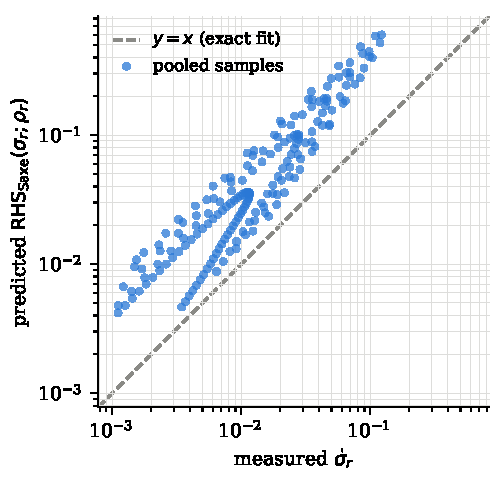
\includegraphics[width=0.82\linewidth]{figures/ode-form-scatter.pdf}
\caption{}
\label{fig:ode-form}
\end{subfigure}

\vspace{6pt}
\begin{subfigure}[t]{\linewidth}
\centering
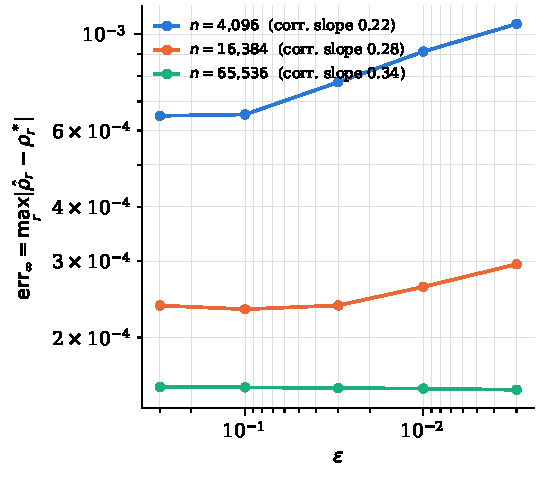
\includegraphics[width=0.82\linewidth]{figures/rate-isolation.pdf}
\caption{}
\label{fig:rate-isolation}
\end{subfigure}
\end{minipage}%
};
\end{tikzpicture}
\caption{\textbf{Left:} \textsc{PlateauRecover}, signed-spectrum recovery from a linear
JEPA training run. Step~2 is the only call to sample covariances; Steps~3--6 (positive
branch) operate on the trajectory alone. Cost $O(nd^2 + T_{\max} d^3)$; implementation
in \nolinkurl{experiments/plateau_recover_corrected.py} of the companion repository.
\textbf{Right, top (a):} diagonal-ODE direction check (\S\ref{ssec:exp-ode-form}),
$\eps=0.05$, $d=6$, pooled over $191$ in-motion samples across six features --- points
sit consistently above $y=x$ (median relative residual $0.74$, max $0.86$, normalised
by $|\mathrm{RHS}_{\mathrm{Saxe}}|$): correct sign and order of magnitude, not a tight
quantitative fit. \textbf{Right, bottom (b):} rate-isolation sweep
(\S\ref{ssec:exp-rate}), $d=10$, $80{,}000$ steps, 3 seeds per point:
$\mathrm{err}_\infty = \max_r|\rhohat-\rhostar|$ vs.\ $\eps$, one curve per $n$;
annotated slope is the polynomial fit of $\log\mathrm{err}_\infty - \log|\log\eps|$
against $\log\eps$ (theory: $0.50$). Both restricted to $L=2$, positive branch.}
\label{alg:plateau-recover}
\end{figure}

\subsection{Empirical validation}
\label{sec:experiments}

We report two synthetic experiments, both restricted to the
\emph{positive branch} ($\rhostar > 0$). Experiment~1 sanity-checks the
diagonal-amplitude ODE \eqref{eq:diagonal-ode} of \S\ref{sec:diagonal-ode}
against direct numerical integration of the JEPA gradient flow.
Experiment~2 isolates the $\eps^{1/L}|\log\eps|$ dynamics-error rate of
Proposition~\ref{prop:plateau} from the $O_p(n^{-1/2})$ sample-noise floor of
Corollary~\ref{cor:finite-sample-end}.

\subsubsection{Setup}
\label{ssec:exp-setup}

In both experiments (with separate configurations) we generate synthetic $(x, y)$ samples from a
ground-truth pencil $(\Syx, \Sxx) \in \RR^{d \times d}$ with prescribed
generalised eigenvalues $\rho_1^* > \rho_2^* > \cdots > \rho_d^*$ on the
positive branch. We train a depth-$L = 2$ JEPA with aligned balanced
initialisation $\Wbar(0) = V(0) = \eps \cdot I$ at the prescribed $\eps$
by full-batch SGD; plateau detection uses a rolling window with a
relative-tolerance stopping rule. Experiment~2 (rate isolation)
uses $d = 10$, the linear spectrum sweep $\rhostar = 1.0, 0.91, 0.82,
\ldots, 0.20$, learning rate $0.05$, and up to $80{,}000$ steps with a
$50$-step/$5 \times 10^{-4}$ plateau window
(\nolinkurl{experiments/plateau_recover_corrected.py} and
\nolinkurl{experiments/rate_isolation_probe.py} of the companion repo).
Experiment~1 (ODE-form sanity check) uses a smaller $d = 6$ configuration
with learning rate $0.02$ for $40{,}000$ steps
(\nolinkurl{experiments/ode_form_fit.py} of the companion repo). It
only needs to verify the ODE's functional form, not exercise the
full-scale sweep.

\subsubsection{Experiment 1: diagonal-ODE sanity check}
\label{ssec:exp-ode-form}

We first compare the trajectory's measured velocity against the diagonal
ODE's predicted right-hand side, evaluated at the empirical
$\sigma_r(t)$:
\[
\mathrm{RHS}_{\mathrm{Saxe}}(\sigma; \rho)
:= L \mu_r \sigma^{2-1/L} (\rho - \sigma^L).
\]
Figure~\ref{fig:ode-form} shows all six features with the correct sign.
The residual is far larger than the $\approx 0.032$
Proposition~\ref{prop:diagonal-ode} predicts. We attribute this gap to
an unresolved scaling constant we have not derived.

\subsubsection{Experiment 2: rate isolation}
\label{ssec:exp-rate}

This experiment checks whether the estimator's error shrinks at the
theoretical rate as $n$ grows:
\[
\mathrm{err}_\infty = O(\eps^{1/L}|\log\eps|) + O_p(n^{-1/2}/\delta),
\]
dynamics term plus sample-noise floor, $1/L = 0.5$ at $L=2$.
Figure~\ref{fig:rate-isolation}: error shrinks about $4\times$ from
$n=4{,}096$ to $65{,}536$, tracking the predicted noise floor. Raw
slopes move from $-0.11$ toward $0$ as $n$ grows, masking the underlying
rate. Correcting for the log factor, slopes rise from $0.22$ to $0.34$,
approaching the theoretical $0.50$.

We attribute this to noise-floor saturation as predicted by Corollary~\ref{cor:finite-sample-end}. Pinning the corrected slope to within
$\pm 0.05$ of $0.50$ needs another order of magnitude beyond $n=65{,}536$.
We leave this and a real-data demonstration to follow-on work.

